\section{Prototyping}
Prototypes and sketches were used to envision design ideas within the \localgroup{}, and for gathering feedback from customers. 
This worked well with the iterative work process of the project, and new prototypes and sketches were continuously built on top of existing ones.

Later prototypes were used to demonstrate the design of the product to the customers. 
These prototypes were implemented on paper, and showed the different screens of the product while demonstrating the control flow of the system in specific use cases. 
This was important in evaluating the design, and gave reassurance about the quality of the design. 

An example of a prototype can be seen in \autoref{fig:first-prototype}

\begin{figure}[h!]
	\centering
	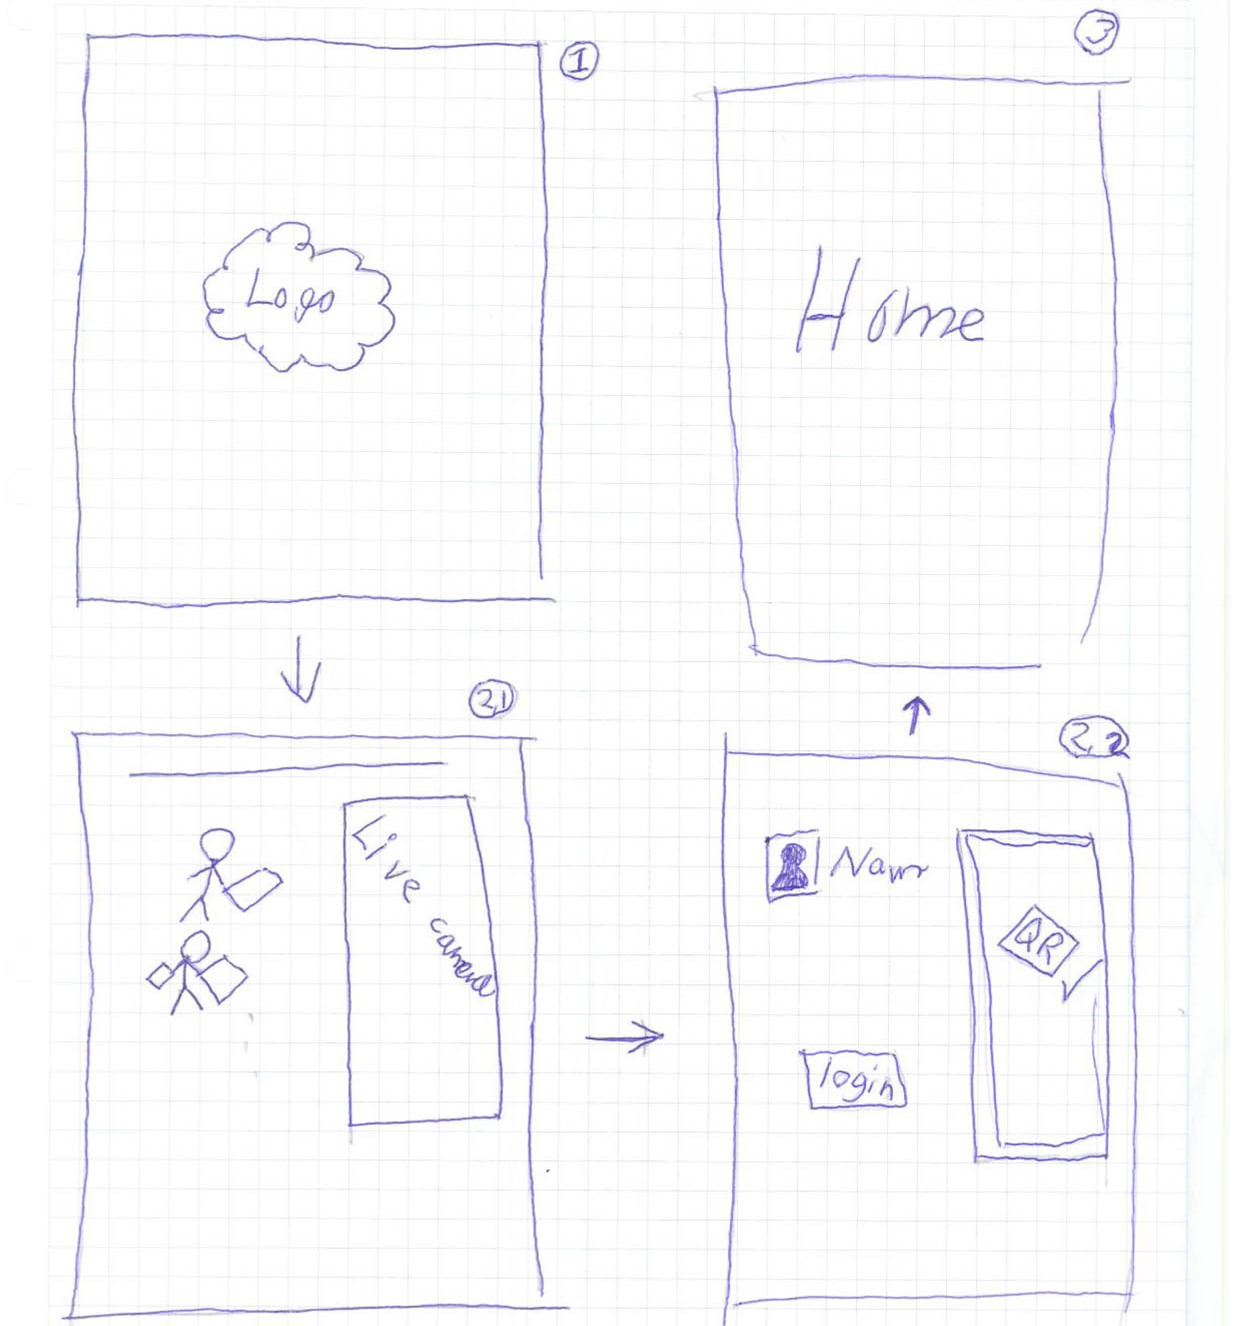
\includegraphics[scale=0.5]{gfx/first-prototype.pdf}
	\caption{Sample prototype}
	\label{fig:first-prototype}
\end{figure}